\documentclass[11pt,a4paper]{article}

\usepackage[margin=22mm]{geometry}
\usepackage{booktabs}
\usepackage{graphicx}
\usepackage{float}
\usepackage[hidelinks]{hyperref}

\graphicspath{{../plots/crds_180s_flush_60s_sensitivity_v01/}}
\setlength{\parindent}{0pt}
\setlength{\parskip}{0.65em}
\renewcommand{\arraystretch}{1.12}

\title{Sensitivity analysis of a 180-s CRDS flush followed by a 60-s average}
\author{High-resolution gas concentration mapping workflow}
\date{21 August 2026}

\begin{document}
\maketitle

\begin{abstract}
This reproducible sensitivity analysis reprocessed all four measurement campaigns using a 180-s CRDS line-flushing period followed by a 60-s concentration average. The average was assigned to the fourth minute of each nominal 240-s valve dwell and was harmonised with the existing FTIR observations. Means, medians, standard deviations, coefficients of variation (CV), block-wise leave-one-out relative errors (LOO RE), and spatial-temporal mixed models were recalculated for CO$_2$, CH$_4$, NH$_3$, and three dimensionless gas ratios. Temporal two-hour blocks explained most of the modelled variation in CO$_2$ and CH$_4$. Spatial variation was more prominent for NH$_3$, particularly in Campaigns 2 and 3. Changing the CRDS averaging window altered campaign-level gas means by analyser-dependent amounts, with the largest median change observed for NH$_3$ in Campaign 1 and CH$_4$ in Campaign 2. The results are a processing sensitivity assessment and do not replace the primary manuscript analysis without a documented methodological decision.
\end{abstract}

\section{Purpose and scope}

The analysis tests the consequences of allowing three minutes for sample transport and line equilibration before retaining the final minute of every nominal four-minute CRDS valve position. It covers Campaigns 1--4. It also provides one harmonised data frame containing FTIR and CRDS observations with the established campaign-specific sampling-point mapping. Shannon entropy was deliberately excluded.

\section{Data preparation}

Per-second CRDS files were read from the recovered Picarro archives. Cyclic experimental periods were identified from the expected MPVPosition sequences. Within each accepted valve dwell, records from 0 to less than 180~s were discarded and records from 180 to less than 240~s were averaged. A minimum of 30 retained raw records and an observed dwell of at least 230~s were required. The timestamp was assigned to the whole minute containing the last retained record, representing the fourth minute of the dwell. Thus, the nominal interval remained 240~s.

FTIR observations were not re-averaged. Their native selector-level timestamps and Messstelle values were retained and sampling points were mapped using the same campaign metadata as the CRDS data. Campaign 1 FTIR values were harmonised to the CRDS scale by dividing CO$_2$ and CH$_4$ by 1.06 and NH$_3$ by 1.09. CRDS concentrations and H$_2$O were not corrected. The combined output preserves raw, corrected, and analysis-scale columns.

Only missing, zero, and negative response values were excluded response-wise from statistics. No IQR filter or other statistical outlier removal was applied. The background point \texttt{s} and the ring-line level \texttt{ring\_in} remain in the combined data but were excluded from internal spatial comparisons.

\begin{table}[H]
\centering
\caption{Prepared analyser observations. The number of sampling points includes retained background or ring-line levels, where applicable. The FTIR records have no CRDS raw-record count.}
\small
\begin{tabular}{llrrr}
\toprule
Campaign & Analyser & Observations & Levels & Median raw records\\
\midrule
1 & FTIR1 & 39,861 & 10 & --\\
1 & FTIR2 & 40,020 & 10 & --\\
1 & CRDS8 & 21,219 & 16 & 69\\
1 & CRDS9 & 30,155 & 16 & 79\\
2 & CRDS8 & 16,389 & 16 & 70\\
2 & CRDS9 & 16,428 & 16 & 79\\
2 & FTIR2 & 83 & 3 & --\\
3 & CRDS8 & 28,903 & 16 & 61\\
3 & CRDS9 & 29,580 & 18 & 79\\
4 & CRDS8 & 57,871 & 9 & 71\\
\bottomrule
\end{tabular}
\end{table}

\section{Statistical analysis}

The arithmetic mean, median, standard deviation (SD), median absolute deviation, and CV were calculated for each response. The CV was defined as
\[
\mathrm{CV}=100\frac{\mathrm{SD}(Y)}{\overline{Y}}.
\]
The ratios NH$_3$/CO$_2$, CH$_4$/CO$_2$, and NH$_3$/CH$_4$ were calculated as dimensionless concentration ratios and were not multiplied by 100.

Sequential observations were assigned to clock-aligned two-hour blocks. A sampling-point median was calculated in each block. For sampling point $i$, the leave-one-out reference was the median of all other internal sampling points available in the same campaign, response, and block. The signed relative error was
\[
\mathrm{LOO\ RE}_{i,t}=100\frac{Y_{i,t}-\widetilde{Y}_{-i,t}}{\widetilde{Y}_{-i,t}}.
\]
Heatmaps report the median absolute LOO RE over blocks.

Spatial and temporal contributions were evaluated with crossed random-intercept models fitted separately by campaign and response:
\[
\log(Y_{i,t})=\beta_0+b_i+c_t+\varepsilon_{i,t},
\]
where $b_i$ is the sampling-point effect and $c_t$ is the two-hour-block effect. Variance components are presented as percentages of total model variance. Vertical-group relevance was assessed for Campaigns 1--3 by likelihood-ratio comparison of models with and without vertical group as a fixed effect while retaining random intercepts for horizontal position and two-hour block.

\section{Results}

\subsection{Network-level concentrations}

\begin{table}[H]
\centering
\caption{Network-level descriptive statistics after the 180-s flush and 60-s average. Concentrations are in ppm. CV is in percent.}
\small
\begin{tabular}{clrrrrr}
\toprule
Campaign & Gas & $n$ & Mean & Median & SD & CV\\
\midrule
1 & CO$_2$ & 127,267 & 622.77 & 612.26 & 106.94 & 17.17\\
1 & CH$_4$ & 127,270 & 18.76 & 18.02 & 8.10 & 43.19\\
1 & NH$_3$ & 127,189 & 2.09 & 2.01 & 0.77 & 36.85\\
2 & CO$_2$ & 32,873 & 636.80 & 628.11 & 118.27 & 18.57\\
2 & CH$_4$ & 32,873 & 18.37 & 17.47 & 9.67 & 52.66\\
2 & NH$_3$ & 32,873 & 0.86 & 0.79 & 0.39 & 45.75\\
3 & CO$_2$ & 55,187 & 559.36 & 535.69 & 99.98 & 17.87\\
3 & CH$_4$ & 55,187 & 12.11 & 10.37 & 6.95 & 57.36\\
3 & NH$_3$ & 55,187 & 0.70 & 0.61 & 0.39 & 56.35\\
4 & CO$_2$ & 45,010 & 565.68 & 547.14 & 84.48 & 14.93\\
4 & CH$_4$ & 45,010 & 12.37 & 11.04 & 6.43 & 51.97\\
4 & NH$_3$ & 45,010 & 0.60 & 0.55 & 0.30 & 49.89\\
\bottomrule
\end{tabular}
\end{table}

The separation between means and medians was small for CO$_2$ but was larger for CH$_4$ and NH$_3$, consistent with right-skewed concentration distributions. CO$_2$ had the smallest network CV in every campaign. CH$_4$ and NH$_3$ were substantially more variable.

\subsection{Effect of the changed CRDS dwell allocation}

\begin{table}[H]
\centering
\caption{Median analyser-level change in the campaign mean when the former 60-s flush plus 180-s average was replaced by a 180-s flush plus 60-s average. Values are percentages. Ranges show the minimum and maximum analyser-specific changes.}
\small
\begin{tabular}{clrr}
\toprule
Campaign & Gas & Median change & Analyser range\\
\midrule
1 & CO$_2$ & 0.95 & $-0.04$ to 1.95\\
1 & CH$_4$ & 0.69 & $-0.13$ to 1.50\\
1 & NH$_3$ & 5.33 & $-0.28$ to 10.94\\
2 & CO$_2$ & 2.70 & 0.21 to 5.19\\
2 & CH$_4$ & 8.00 & 0.58 to 15.42\\
2 & NH$_3$ & $-1.72$ & $-5.76$ to 2.31\\
3 & CO$_2$ & $-1.52$ & $-1.73$ to $-1.32$\\
3 & CH$_4$ & $-5.34$ & $-6.29$ to $-4.39$\\
3 & NH$_3$ & $-4.34$ & $-4.40$ to $-4.27$\\
4 & CO$_2$ & 1.11 & 1.11 to 1.11\\
4 & CH$_4$ & 3.39 & 3.39 to 3.39\\
4 & NH$_3$ & $-0.37$ & $-0.37$ to $-0.37$\\
\bottomrule
\end{tabular}
\end{table}

The direction and magnitude of the sensitivity were gas-, analyser-, and campaign-dependent. The comparison is not a strictly paired record-level experiment because recovered-file coverage and accepted-cycle coverage can differ between the old and new preparation workflows. It should therefore be interpreted as a pipeline-level sensitivity analysis.

\subsection{Spatial and temporal variance}

\begin{table}[H]
\centering
\caption{Variance partition from crossed mixed models fitted to log-transformed two-hour sampling-point medians. Values are percentages of total model variance.}
\small
\begin{tabular}{clrrr}
\toprule
Campaign & Gas & Spatial SP & Temporal block & Residual\\
\midrule
1 & CO$_2$ & 4.09 & 70.47 & 25.44\\
1 & CH$_4$ & 4.95 & 67.25 & 27.80\\
1 & NH$_3$ & 18.42 & 49.18 & 32.40\\
2 & CO$_2$ & 9.37 & 70.81 & 19.82\\
2 & CH$_4$ & 12.15 & 65.29 & 22.56\\
2 & NH$_3$ & 46.39 & 40.25 & 13.37\\
3 & CO$_2$ & 13.26 & 59.24 & 27.50\\
3 & CH$_4$ & 27.29 & 46.71 & 26.00\\
3 & NH$_3$ & 41.69 & 37.46 & 20.85\\
4 & CO$_2$ & 20.40 & 59.25 & 20.35\\
4 & CH$_4$ & 27.23 & 48.20 & 24.56\\
4 & NH$_3$ & 28.32 & 60.18 & 11.50\\
\bottomrule
\end{tabular}
\end{table}

Temporal blocks accounted for 59.2--70.8\% of CO$_2$ variance and 46.7--67.2\% of CH$_4$ variance. NH$_3$ showed a stronger spatial contribution, reaching 46.4\% in Campaign 2 and 41.7\% in Campaign 3. All six vertical-group likelihood-ratio tests in each of Campaigns 1--3 were significant ($p<10^{-8}$). These tests establish statistical vertical structure, but their large sample sizes mean that effect magnitude must be interpreted from the descriptive plots and variance components rather than from $p$-values alone.

\clearpage
\section{Figures}

\begin{figure}[H]
\centering
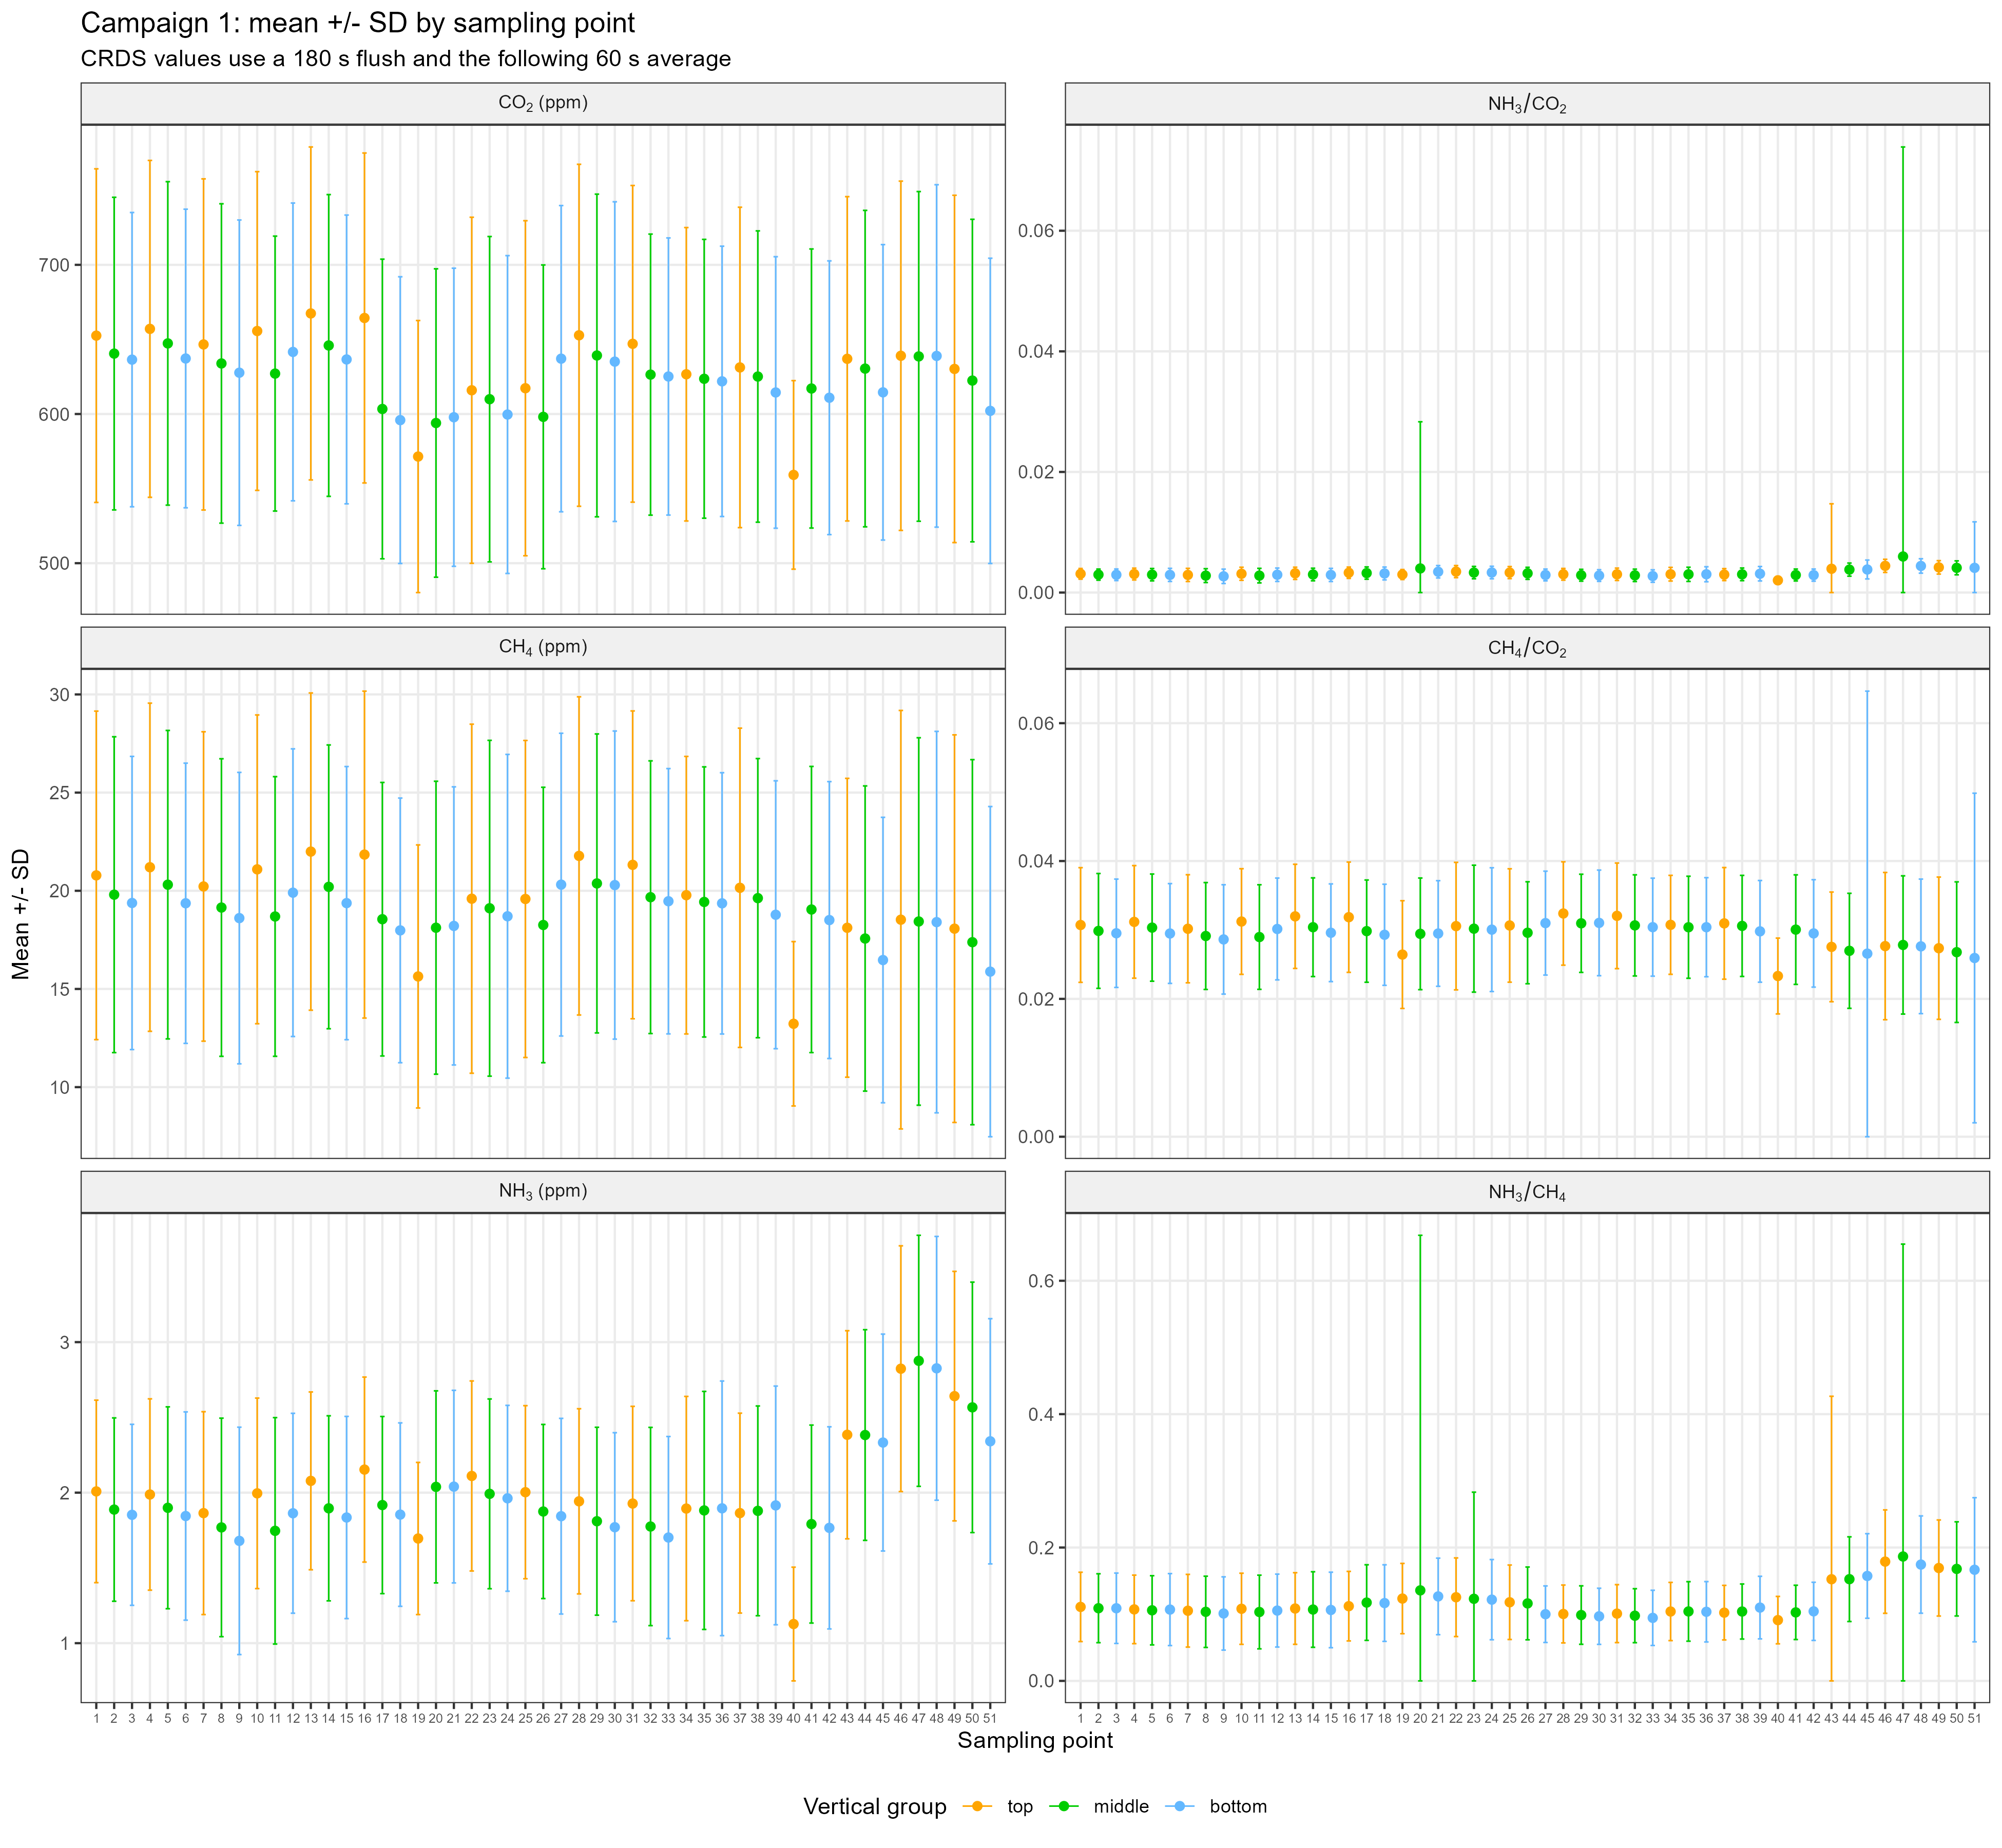
\includegraphics[width=\textwidth]{Fig_mean_SD_campaign1.png}
\caption{Campaign 1 mean $\pm$ SD for each gas and dimensionless ratio at each internal sampling point. Colours identify the top, middle, and bottom vertical groups.}
\end{figure}

\begin{figure}[H]
\centering
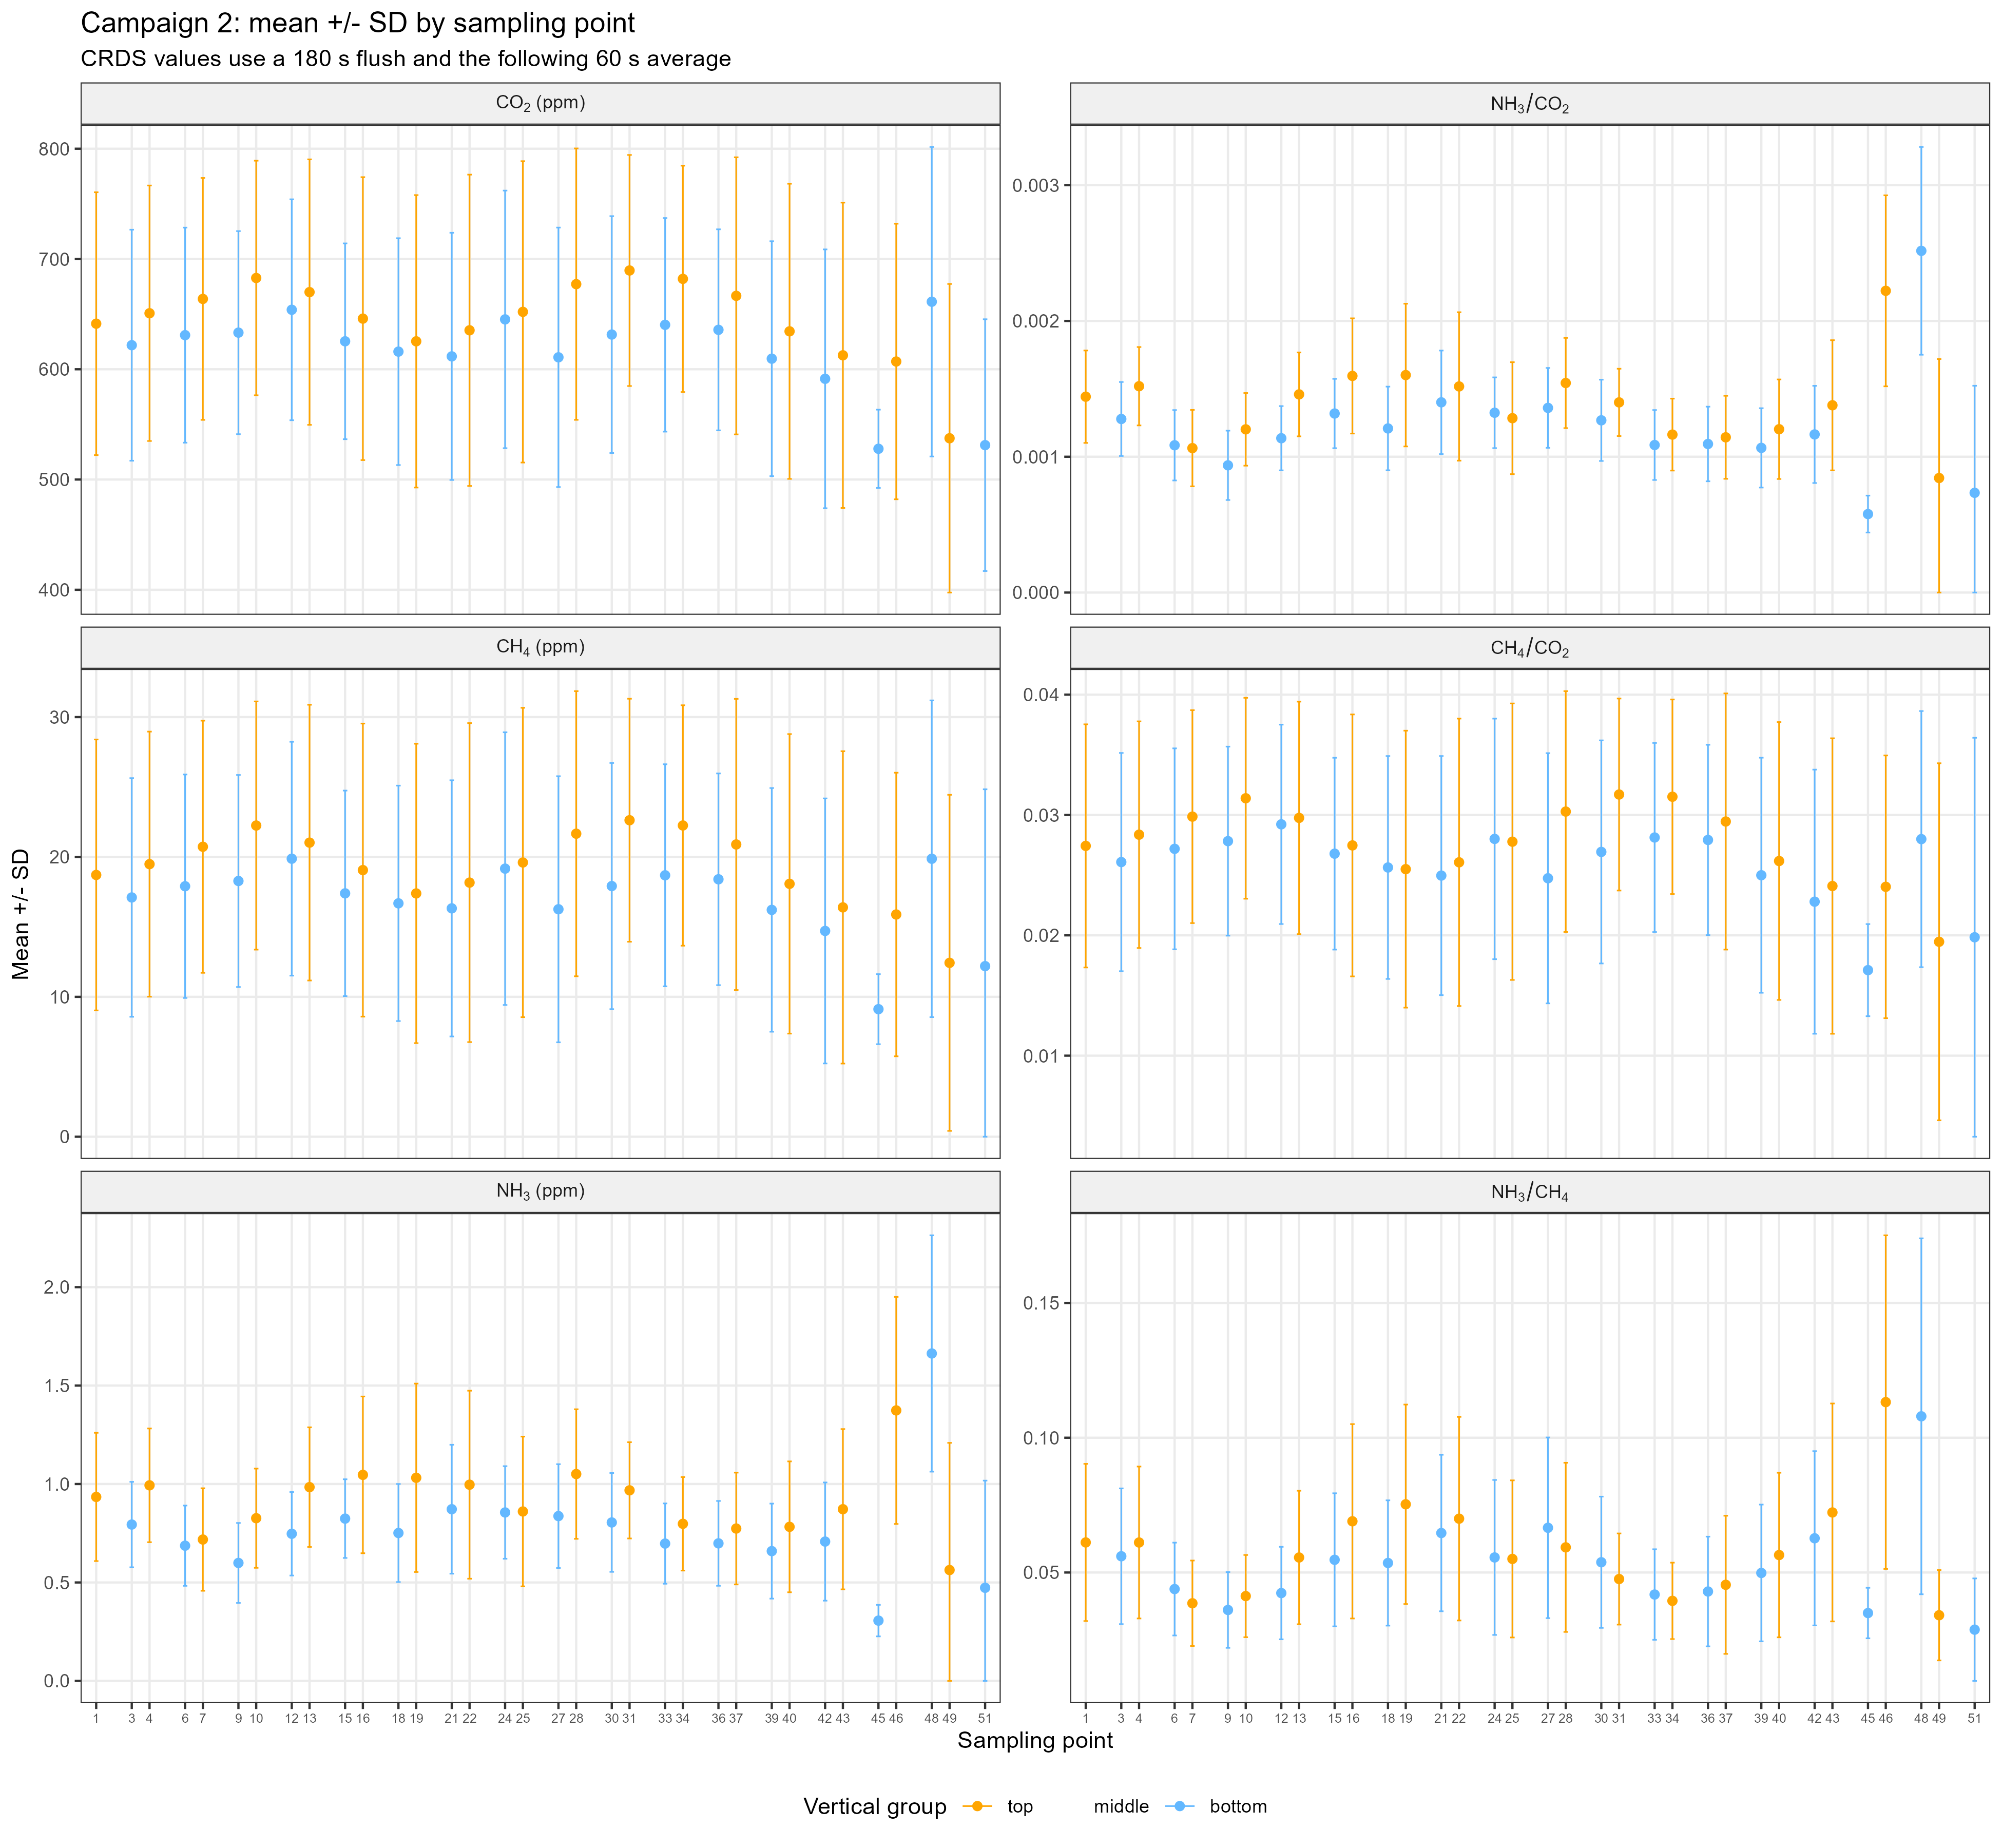
\includegraphics[width=\textwidth]{Fig_mean_SD_campaign2.png}
\caption{Campaign 2 mean $\pm$ SD by internal sampling point. The middle vertical group was not part of the CRDS configuration.}
\end{figure}

\begin{figure}[H]
\centering
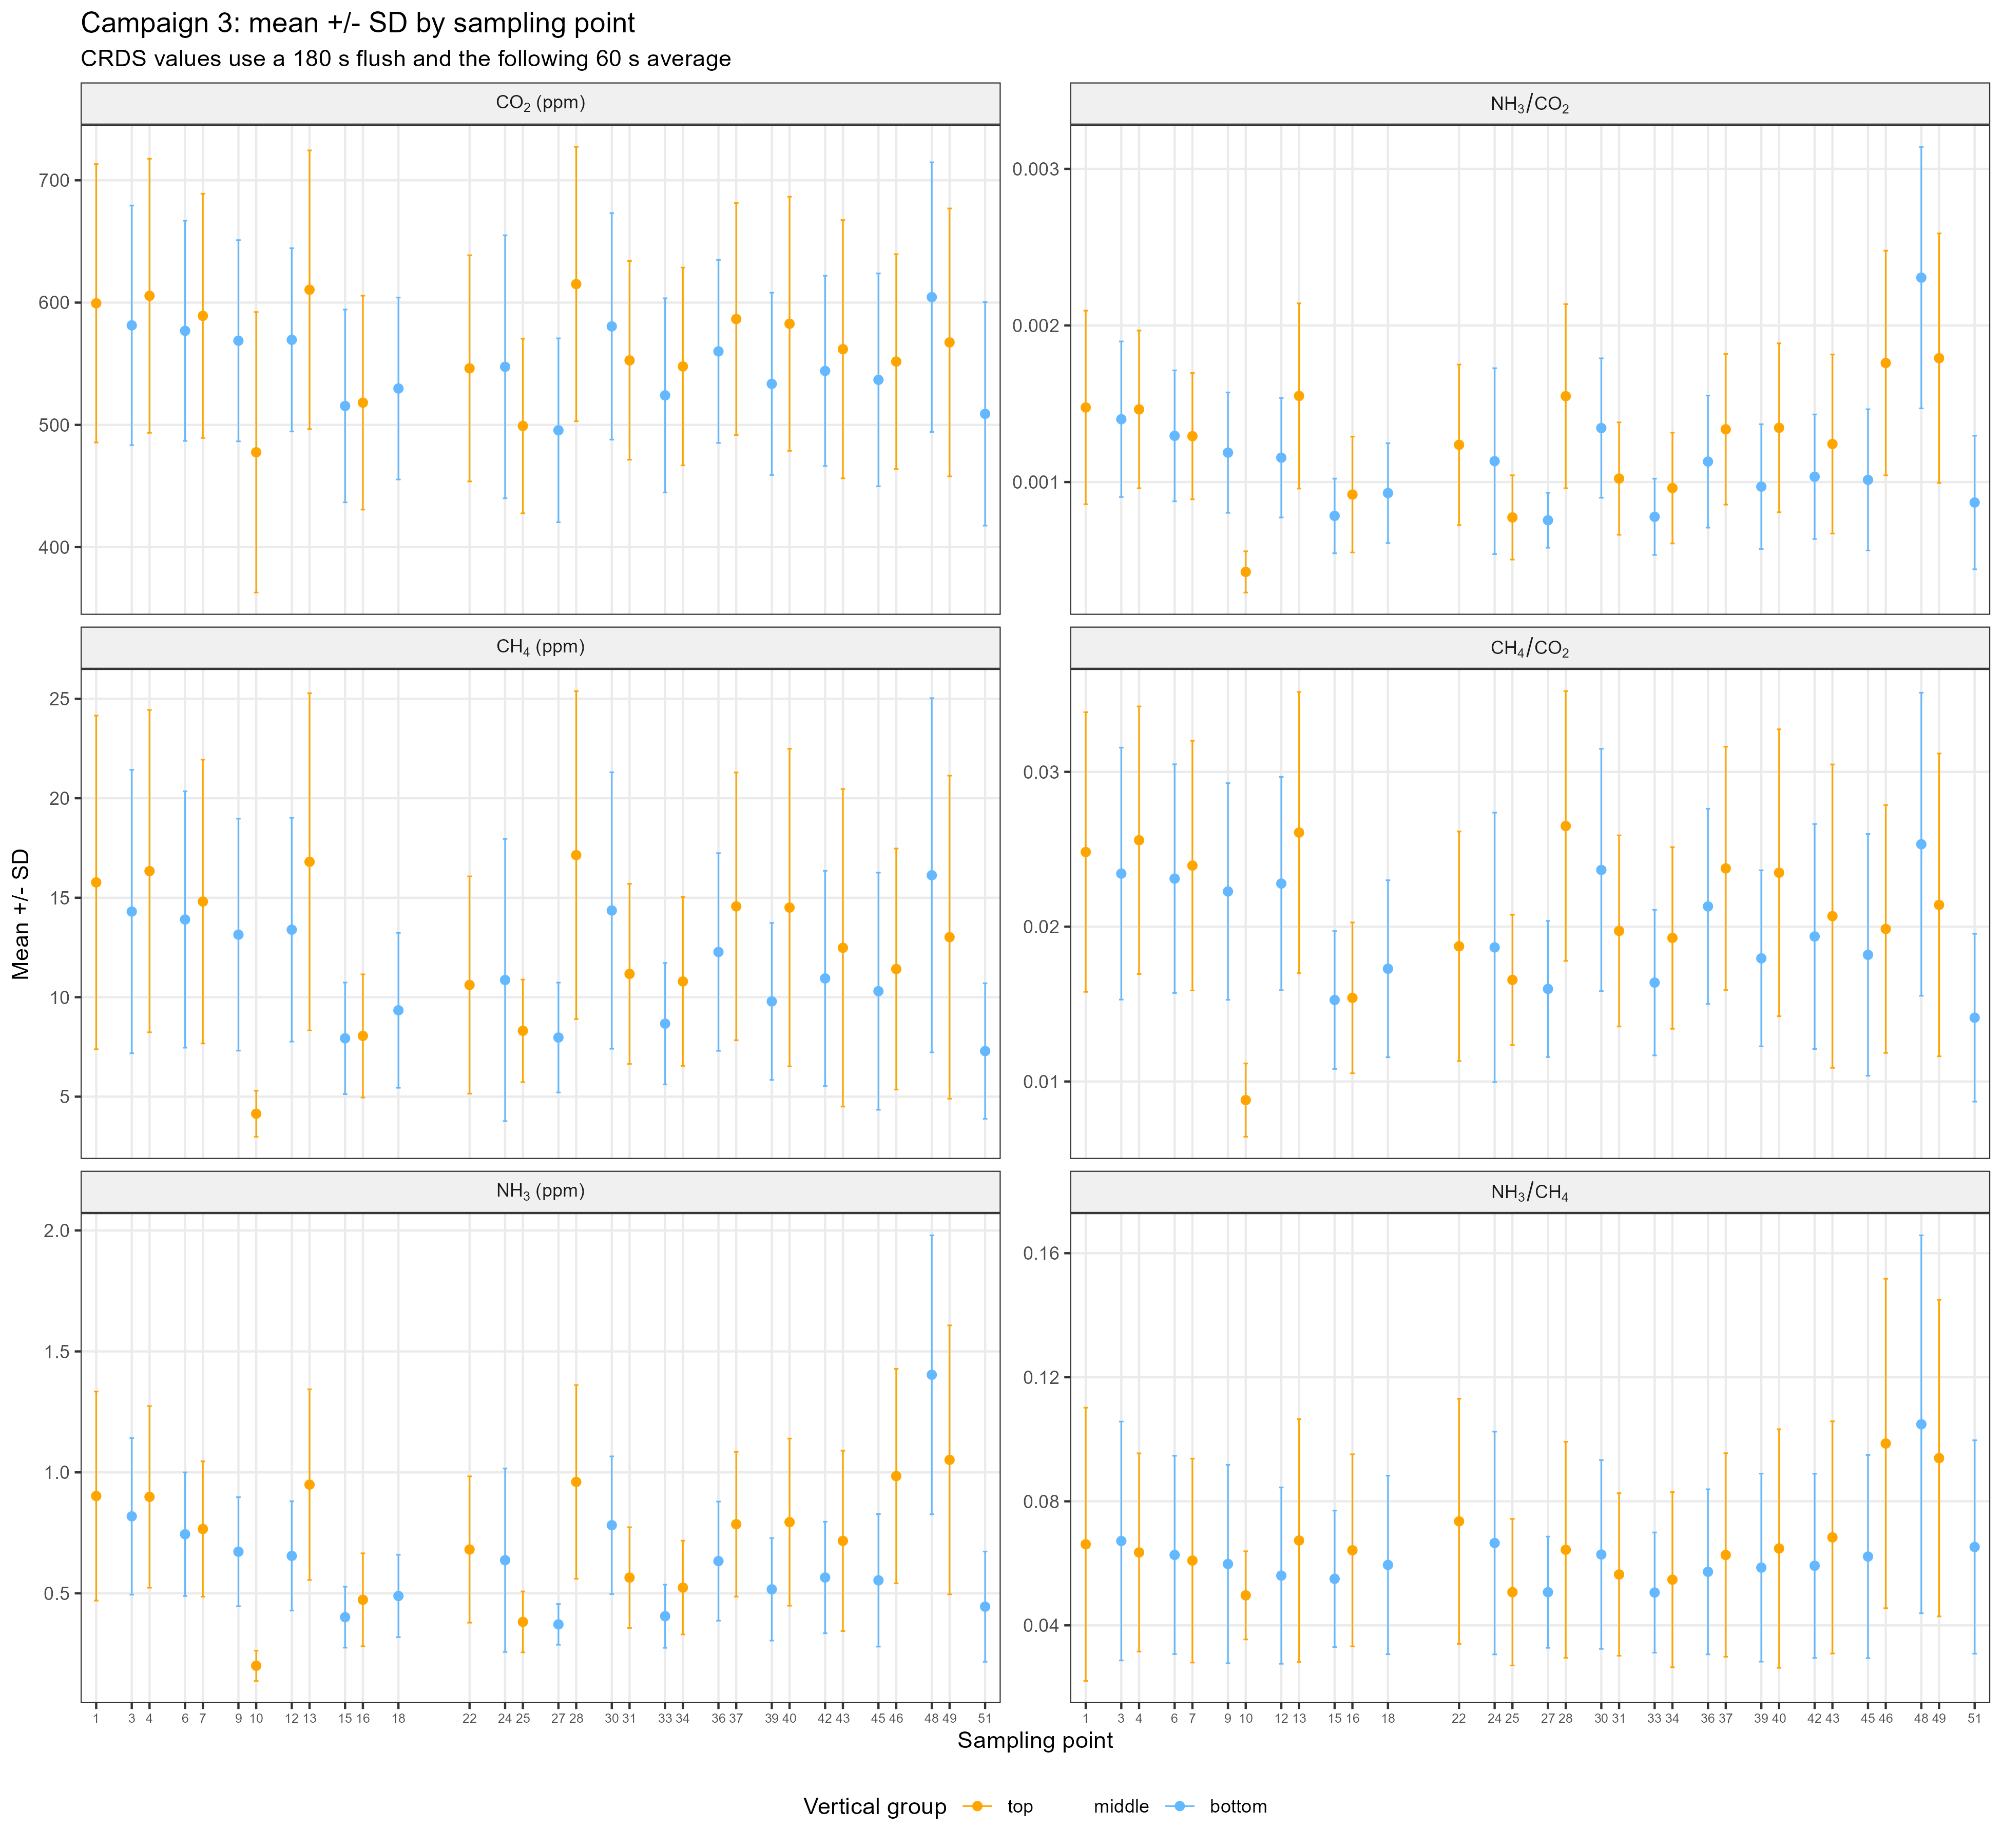
\includegraphics[width=\textwidth]{Fig_mean_SD_campaign3.png}
\caption{Campaign 3 mean $\pm$ SD by internal sampling point.}
\end{figure}

\begin{figure}[H]
\centering
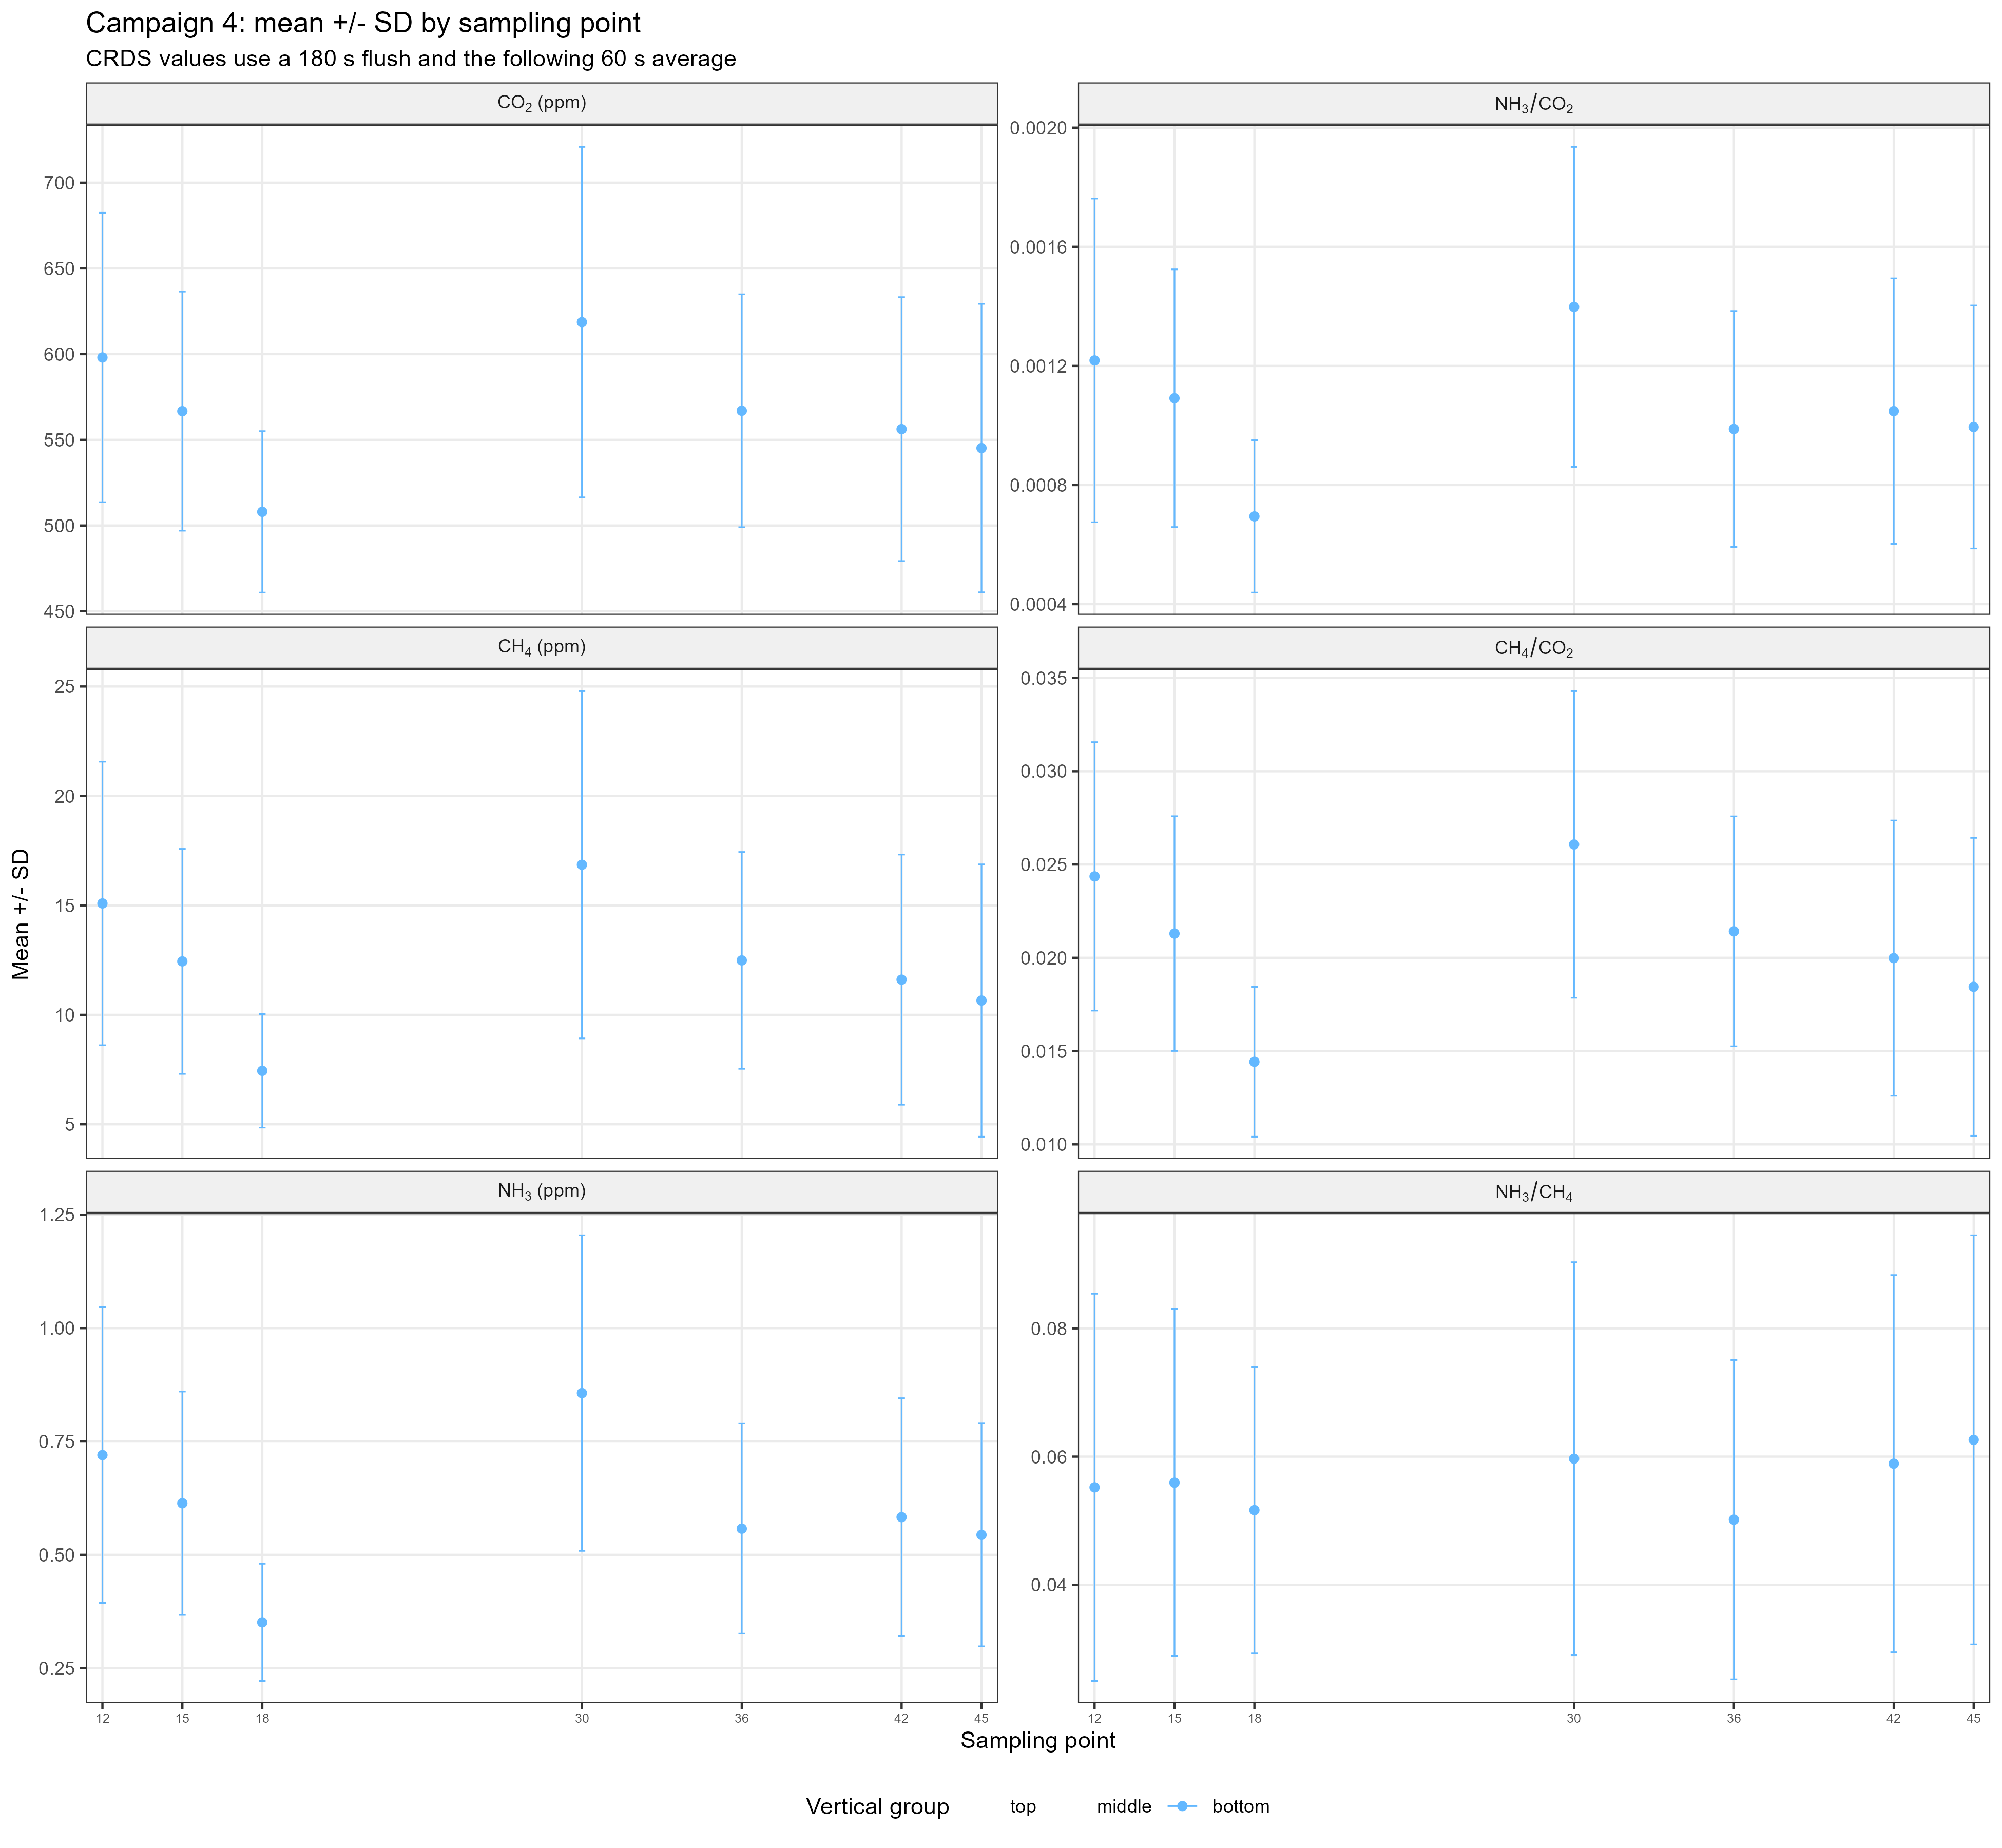
\includegraphics[width=\textwidth]{Fig_mean_SD_campaign4.png}
\caption{Campaign 4 mean $\pm$ SD by internal sampling point.}
\end{figure}

\begin{figure}[H]
\centering
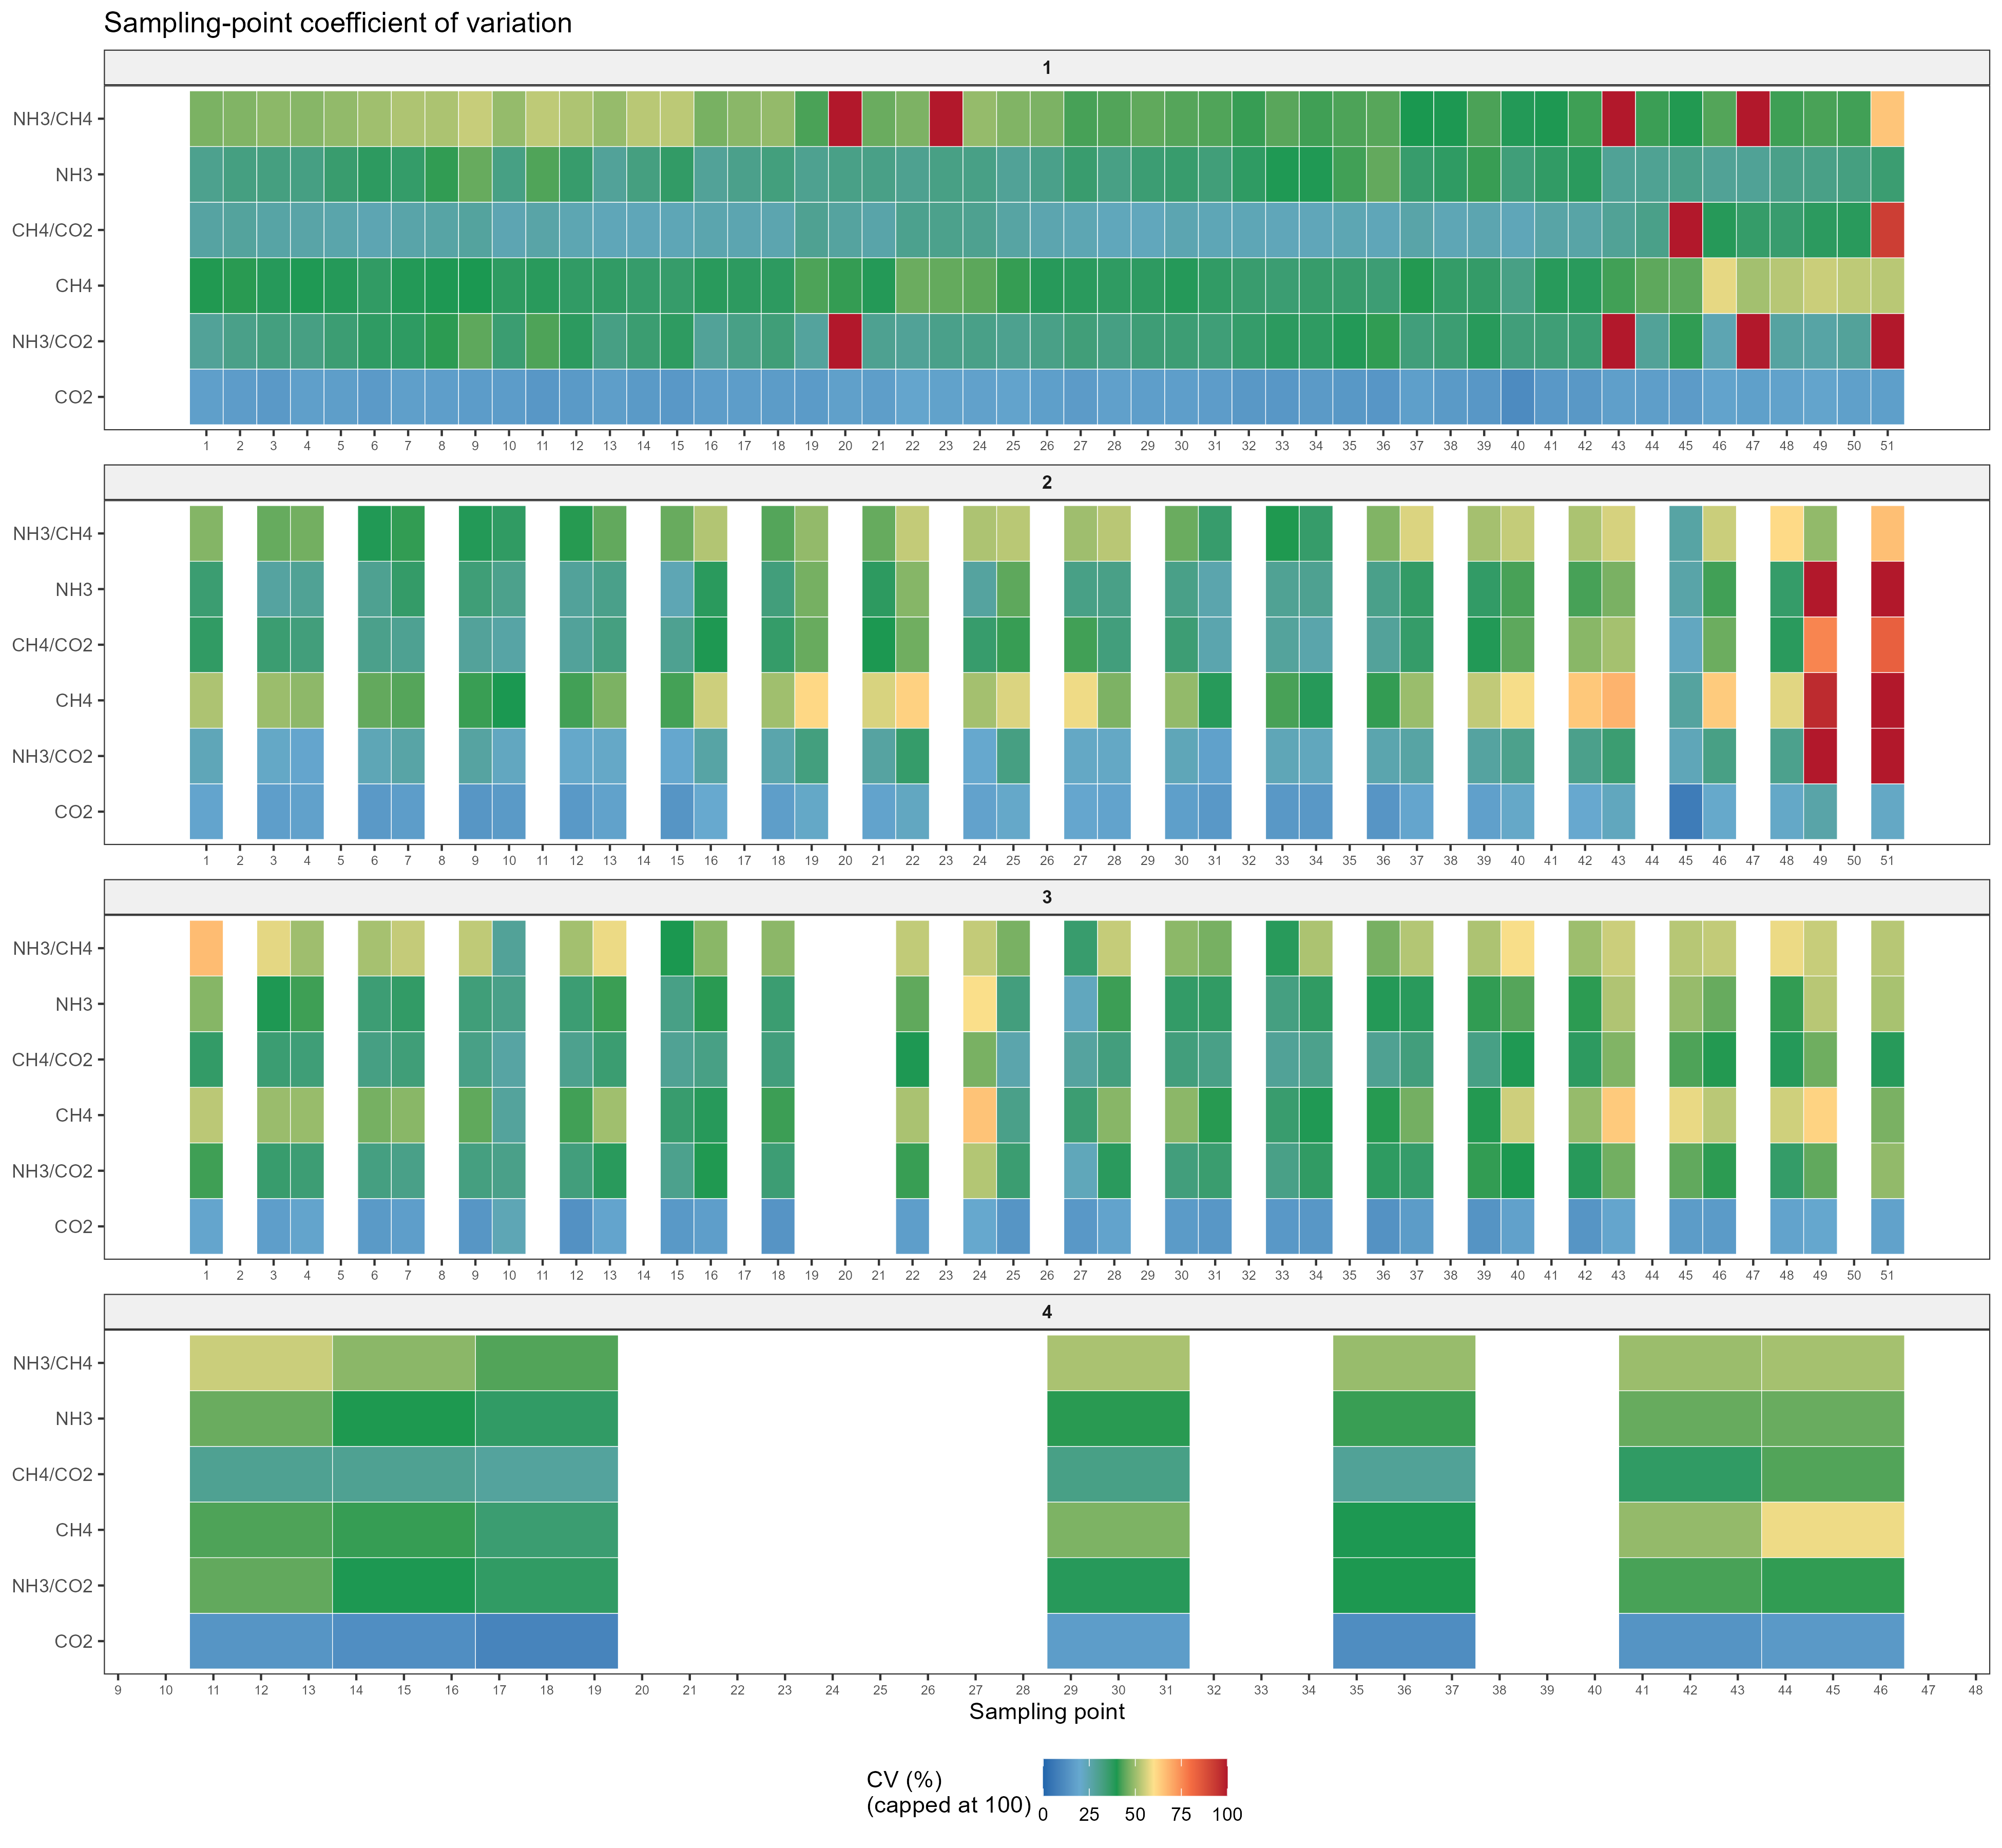
\includegraphics[width=\textwidth]{Fig_CV_heatmaps_campaign1_4.png}
\caption{Sampling-point CV for all gases and ratios. Colour values are capped at 100\% for display only. Uncapped values are retained in the CSV output. Blank cells indicate unmeasured sampling points.}
\end{figure}

\begin{figure}[H]
\centering
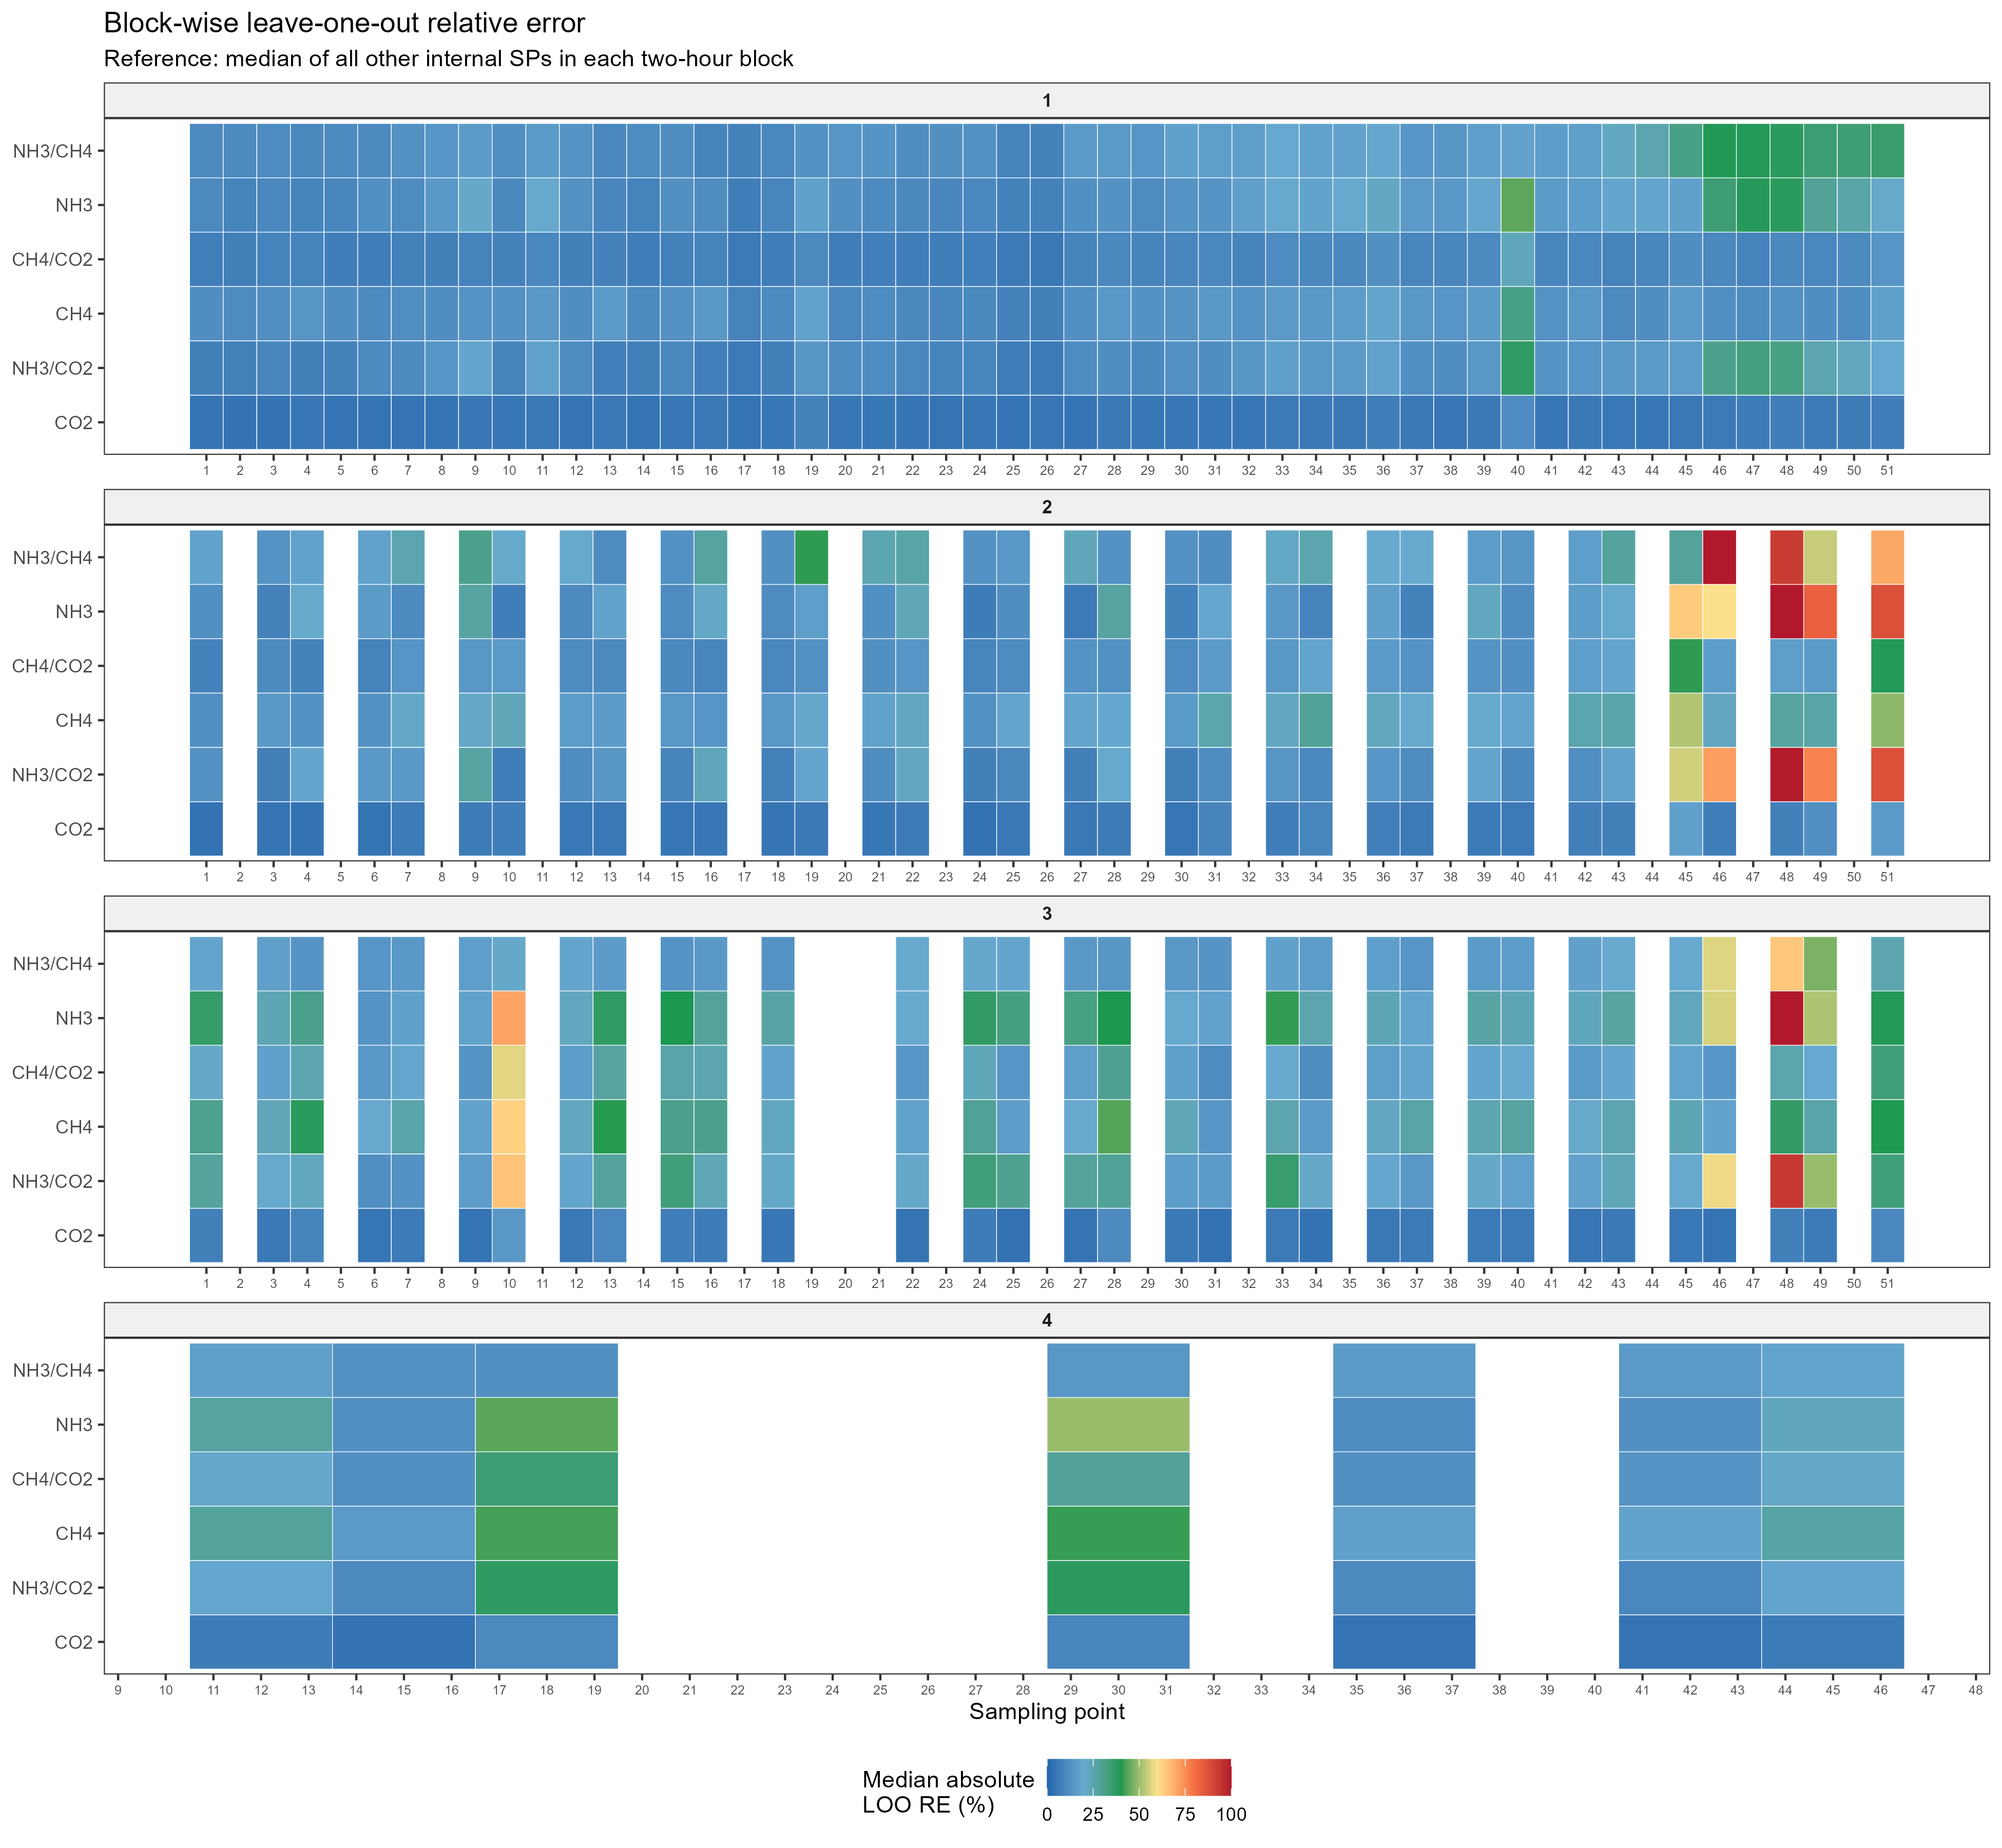
\includegraphics[width=\textwidth]{Fig_LOO_RE_heatmaps_campaign1_4.png}
\caption{Median absolute leave-one-out relative error. Each sampling-point median was compared with the median of all other internal points available in the same two-hour block. Values are capped at 100\% for display only.}
\end{figure}

\begin{figure}[H]
\centering
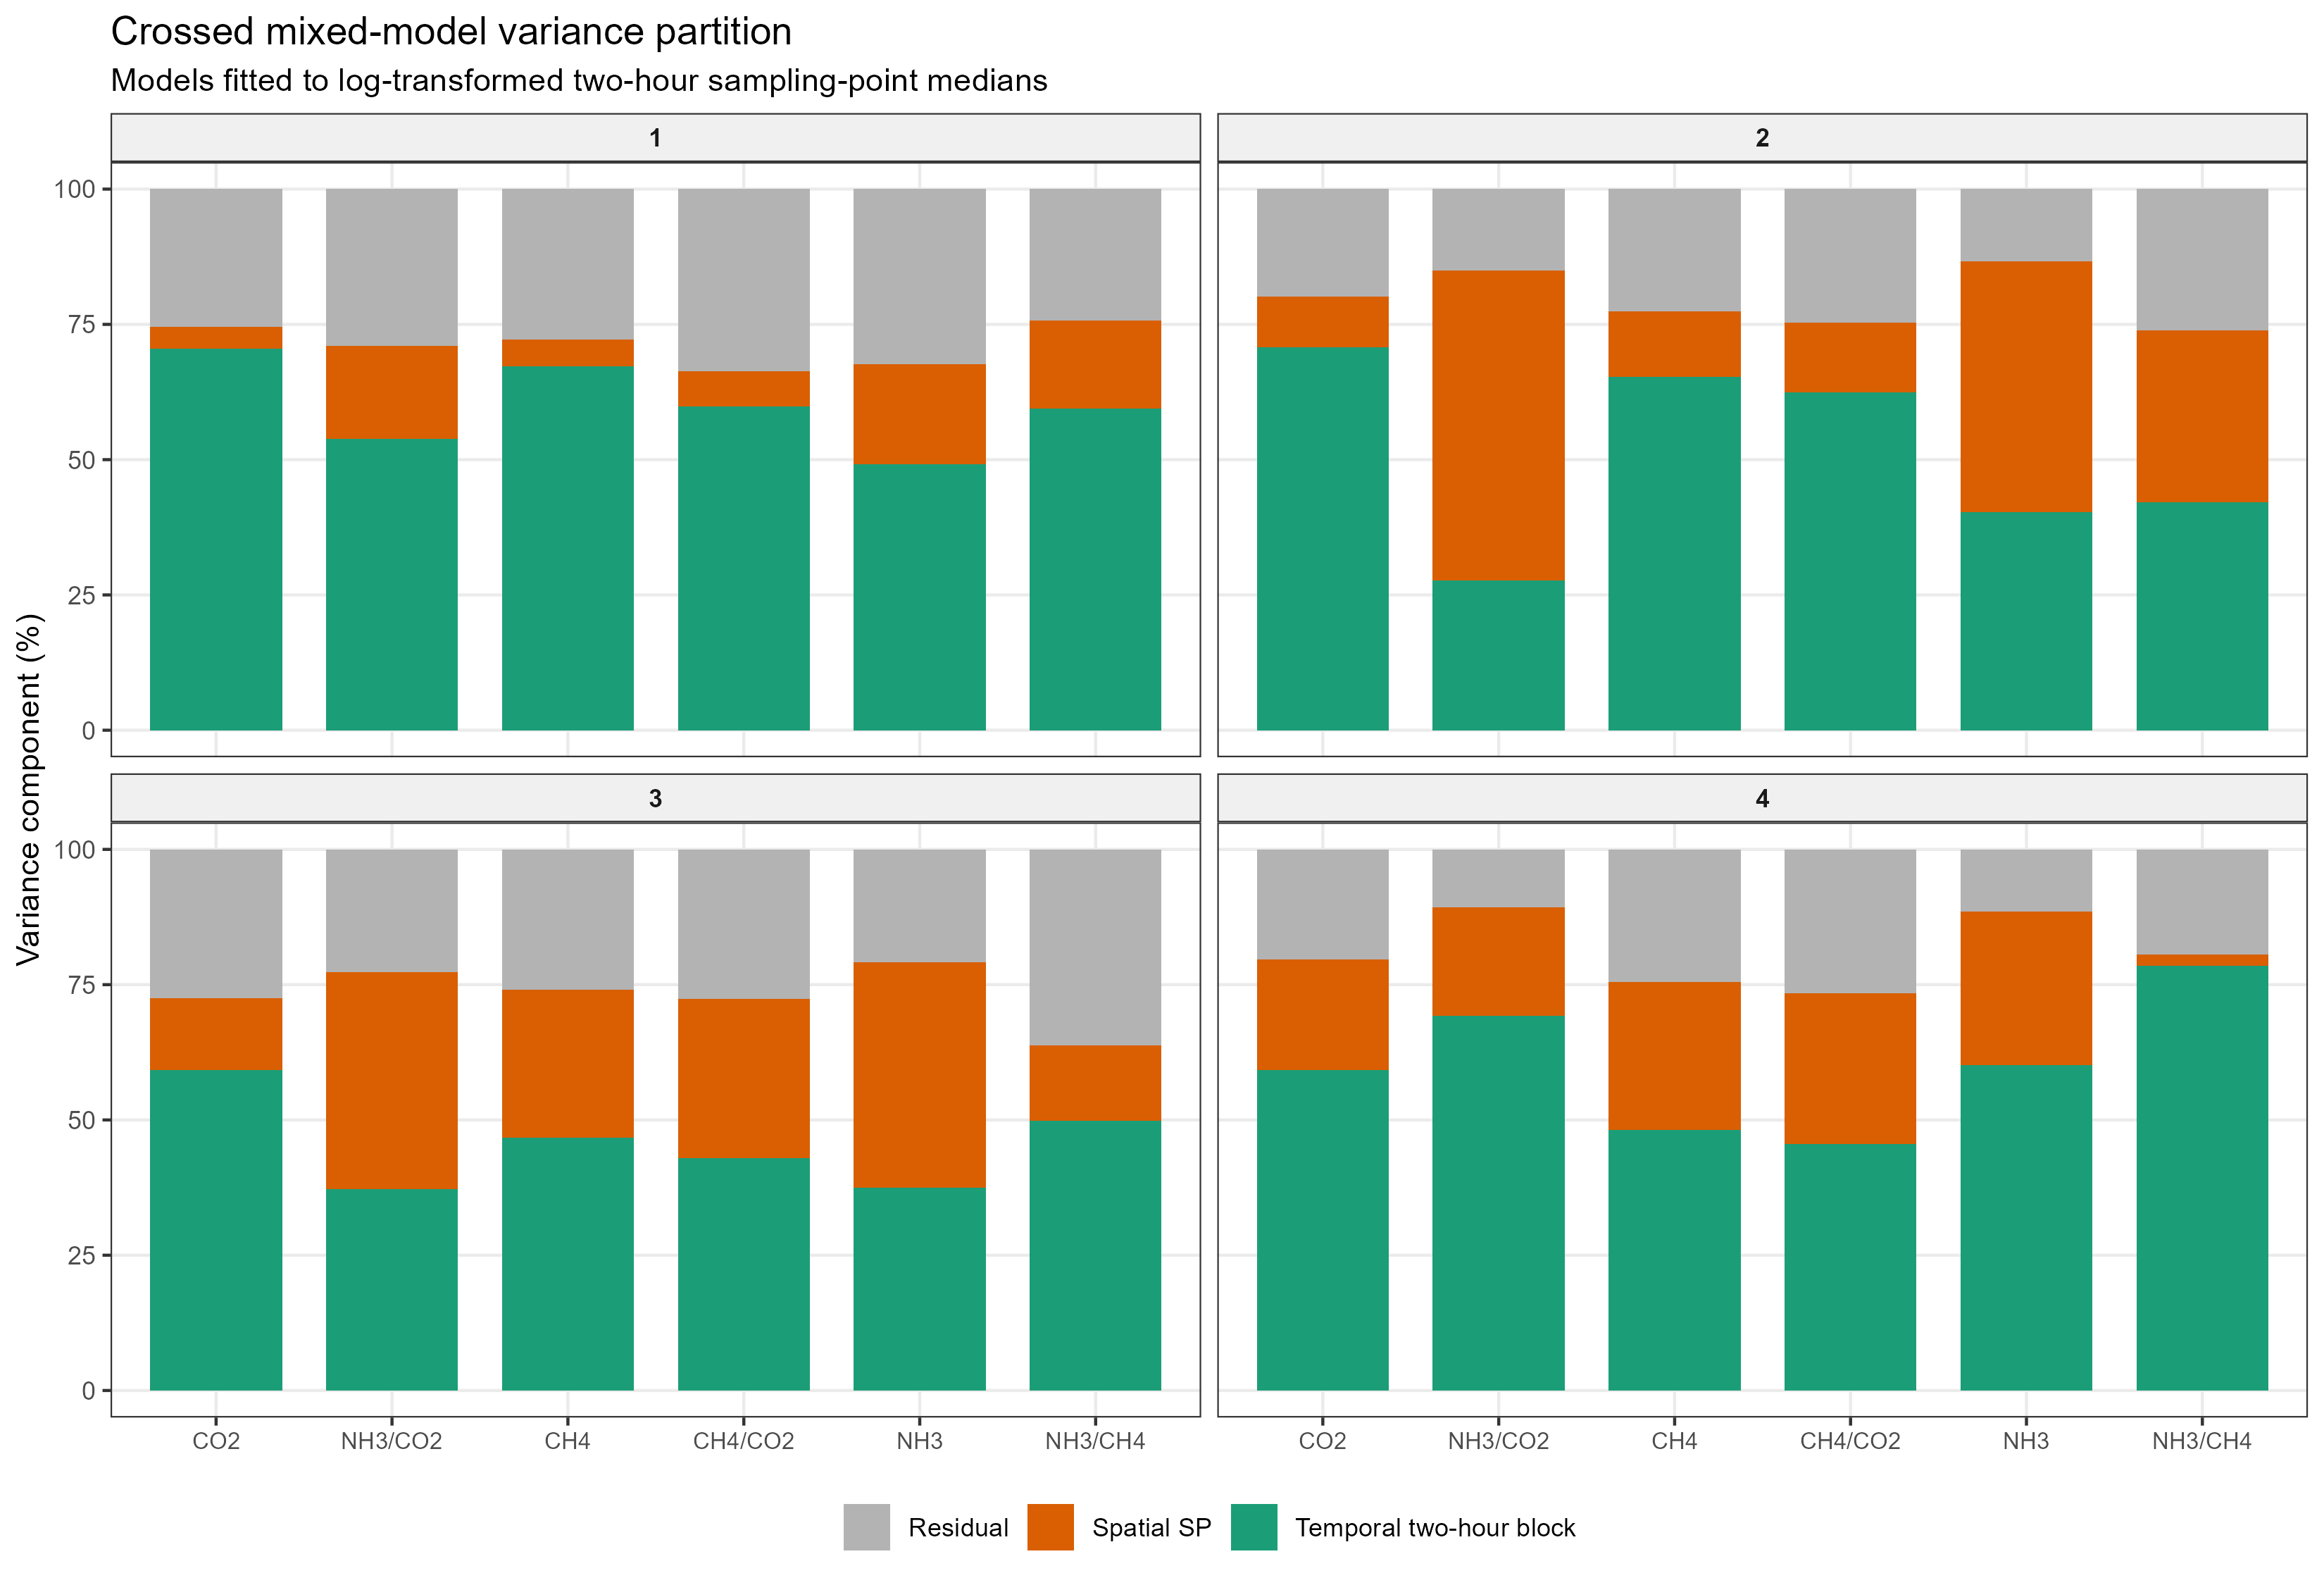
\includegraphics[width=\textwidth]{Fig_mixed_model_variance_partition.png}
\caption{Spatial, temporal, and residual variance percentages from the crossed random-intercept models.}
\end{figure}

\clearpage
\section{Interpretation and limitations}

The 180-s flush plus 60-s averaging rule materially changes some campaign-level estimates, particularly CH$_4$ in Campaign 2 and NH$_3$ in Campaign 1. A final decision should consider physical residence time, analyser response, line length, and stability during the retained minute. The shortened average also increases sensitivity to short-lived peaks.

All positive concentrations were retained as requested. Consequently, very small positive denominator concentrations can produce extreme gas ratios and large ratio SD or CV values. These records are visible in the outputs rather than being hidden by a post-processing threshold. Before using ratios for inference, their corresponding numerator and denominator time series should be reviewed and a physically justified quality rule should be specified prospectively.

Campaign 3 positions that changed function over time were mapped according to the documented switch date. Campaign 4 contains seven internal points plus non-internal line levels. Campaign 2 has sparse FTIR2 coverage. These differences constrain direct comparisons of network density between campaigns. The variance partitions describe the observed data hierarchy. They do not identify causal mechanisms or adjust for weather, management, or animal activity.

\section{Reproducibility}

{\raggedright
The raw-data preparation is implemented in
\path{scripts/04_prepare_crds_180s_flush_60s_average_all_campaigns.R}.
Statistical tables and figures are produced by
\path{scripts/05_crds_180s_flush_60s_statistics_plots.R}.
Prepared measurement CSV files are intentionally excluded from Git. The R scripts, this report source, the compiled PDF, and the plotted PNG files are version controlled.\par}

\end{document}
